\documentclass[conference]{IEEEtran}
\IEEEoverridecommandlockouts

\usepackage{cite}
\usepackage{amsmath,amssymb,amsfonts}
\usepackage{algorithmic}
\usepackage{graphicx}
\graphicspath{{figures/}}
\usepackage{textcomp}
\usepackage{xcolor}
\def\BibTeX{{\rm B\kern-.05em{\sc i\kern-.025em b}\kern-.08em
    T\kern-.1667em\lower.7ex\hbox{E}\kern-.125emX}}
\begin{document}

\title{Multi-Label Speech Emotion Recognition Using 2D CNNs}

\author{\IEEEauthorblockN{Brian Pho, Thomas Truong, Svetlana Yanushkevich}
\IEEEauthorblockA{\textit{Biometric Technologies Laboratory, Department of Electrical and Computer Engineering}\\
\textit{University of Calgary}, Canada\\
\{brian.pho, thomas.truong, syanshk\}@ucalgary.ca}
}

\maketitle

\begin{abstract}
Current emotion classification systems using machine learning often ignore the multi-label data that comes with databases. In this paper, we address the problem of whether machine learning can be used to detect multiple emotions in speech and how accurate they can identify the emotions present. We created an combined database from four voice emotion-labeled databases and trained a 2D convolutional neural network on it to determine if the model could recognize multiple emotions in a speech sample. The model was able to classify the samples with an accuracy of 50\%. This result shows that it is possible to apply machine learning to the problem of multi-label speech emotion recognition and to achieve a reasonable accuracy.
\end{abstract}

\begin{IEEEkeywords}
speech, emotion, classification, neural networks
\end{IEEEkeywords}

\section{Introduction}

\subsection{Literature Review}

The field of affective computing studies the development of systems that can recognize, interpret, process, and simulate human affects. One subfield of affective computing that we are interested in is speech emotion classification. Classifying speech based on its emotional content is applicable to the development of more user friendly kiosks, more interactive digital assistants such as Siri or Google Assistant, and allows for a better understanding of what parts of speech contribute to its emotional content. One method of classification that has demonstrated great success is deep learning. Specifically, the use of convolution neural networks have proven to be successful at classifying emotions in speech as shown by \cite{}. Current research has successfully applied deep learning to automate this process and achieves an accuracy of 90\% \cite.

However, these models only consider a single emotion per speech sample and are often only trained on one to two databases. This paper extends upon this work by considering the problem of multi-label emotion classification of speech using four databases. The IEMOCAP and CREMA-D databases both include multiple labels for each speech sample but the data is usually discarded by only considering the emotion with the majority votes. We argue that discarding the other emotions results in a less realistic model of emotion classification due to not matching human performance and because it sidesteps the problem of ambiguous samples.

\subsection{Summary}

We approach the problem of multi-label emotion classification by using 2D convolution neural networks to classify speech samples into multiple emotions. We collected four databases, two with mutli-labeled and single-labeled samples, and two with only single-labeled samples. We then combined these four databases into an combined database by processing all of the speech samples into log-Mel spectrograms. These log-Mel spectrograms were then fed into a seven layer neural network consisting of four convolutional layers and three dense layers. After training the neural network, the model achieved a 50\% test accuracy.

The paper is outlined as follows:
\begin{itemize}
	\item Section II details the methodology we use such as the how we combined four databases and the architecture of the neural network.
	\item Section III details the results from training the neural network.
	\item Section IV discusses the results in the context of the field and how future work can improve upon the work.
\end{itemize}

\section{Method}

\subsection{Method Summary}

To determine if a machine learning model could perform multi-label emotion classification on speech, we first need to get speech samples with their labeled emotion. We considered eight databases and chose four based on accessibility and the number of common emotions. Given the variability of emotions in each database and the constraint adding more databases increases the difficulty of controlling the consistency of the samples, we chose the following databases
\begin{itemize}
	\item IEMOCAP \cite{busso_2008}
	\item TESS \cite{dupuis_2011}
	\item RAVDESS \cite{livingstone_2018}
	\item CREMA-D \cite{cao_2014}
\end{itemize}

We specifically picked databases that were spoken in English to keep the language consistent. We combined these four databases for training, validating, and testing the neural network. The combined database is detailed in figures \ref{fig:combined_db_db_split}, \ref{fig:combined_db_emotions}, \ref{fig:combined_db_label_types}.

\begin{figure}[h!]
	\centering
	\hspace{6mm}
	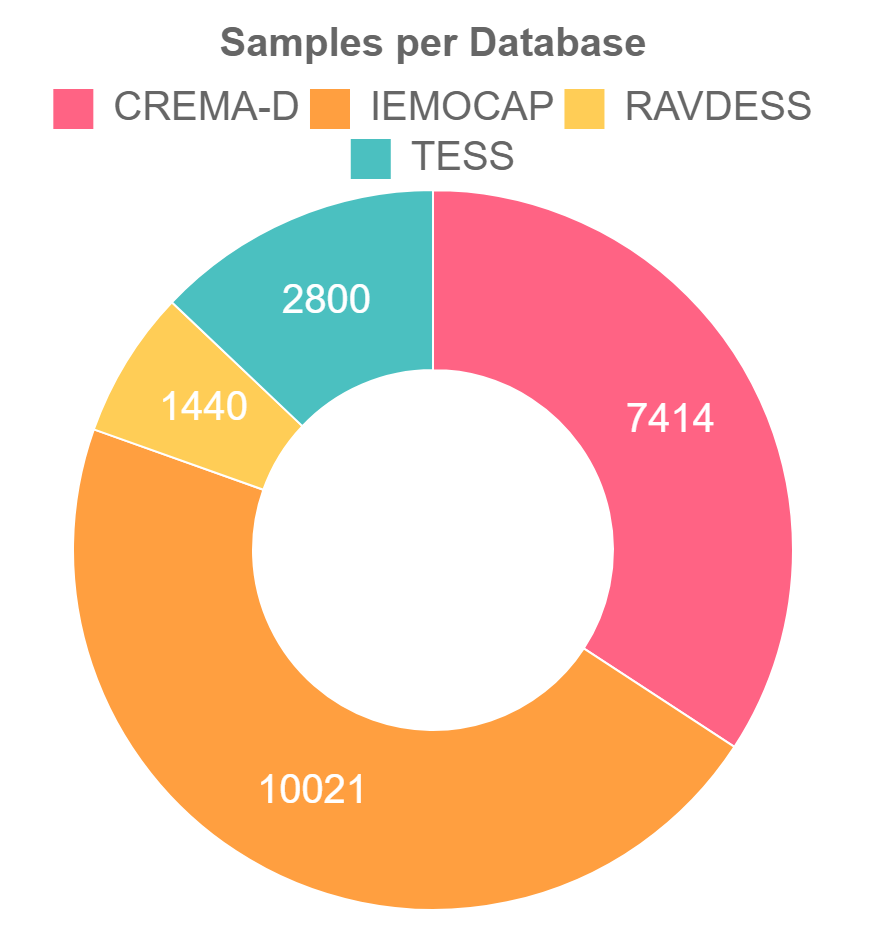
\includegraphics[width=\linewidth]{combined_db_db_split.png} 
	\caption{The proportion of each database in the combined database.}
	\label{fig:combined_db_db_split}
\end{figure}

\begin{figure}[h!]
	\centering
	\hspace{6mm}
	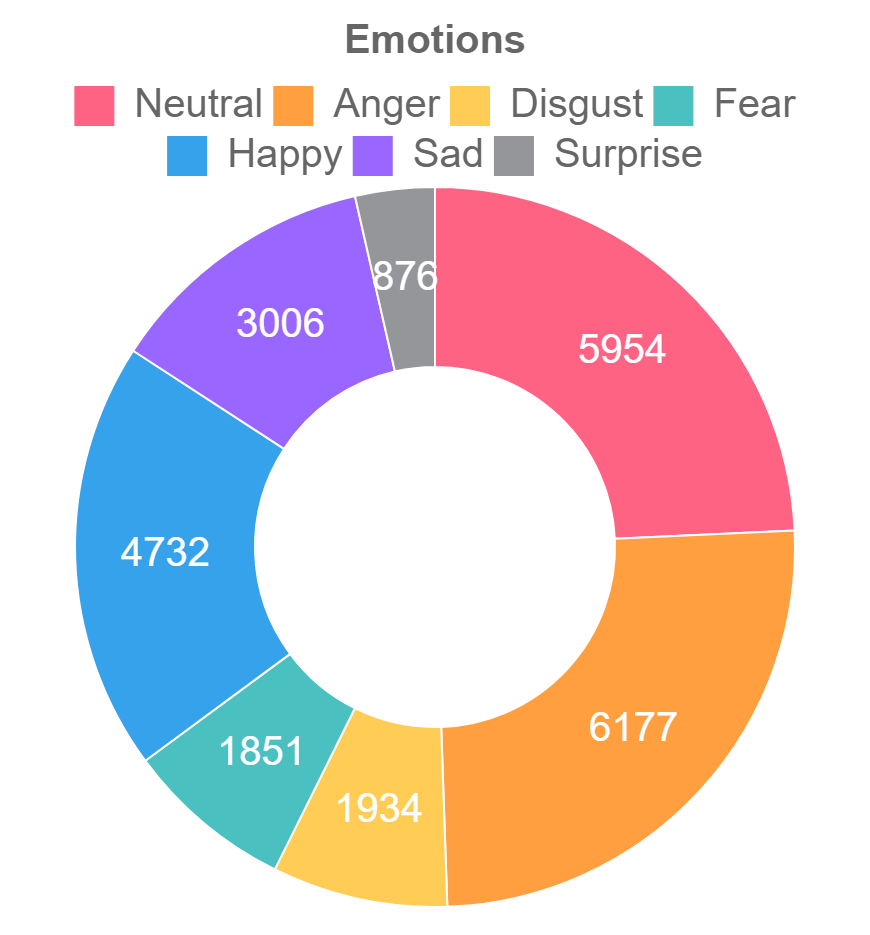
\includegraphics[width=\linewidth]{combined_db_emotions.png} 
	\caption{The proportion of each emotion in the combined database.}
	\label{fig:combined_db_emotions}
\end{figure}

\begin{figure}[h!]
	\centering
	\hspace{6mm}
	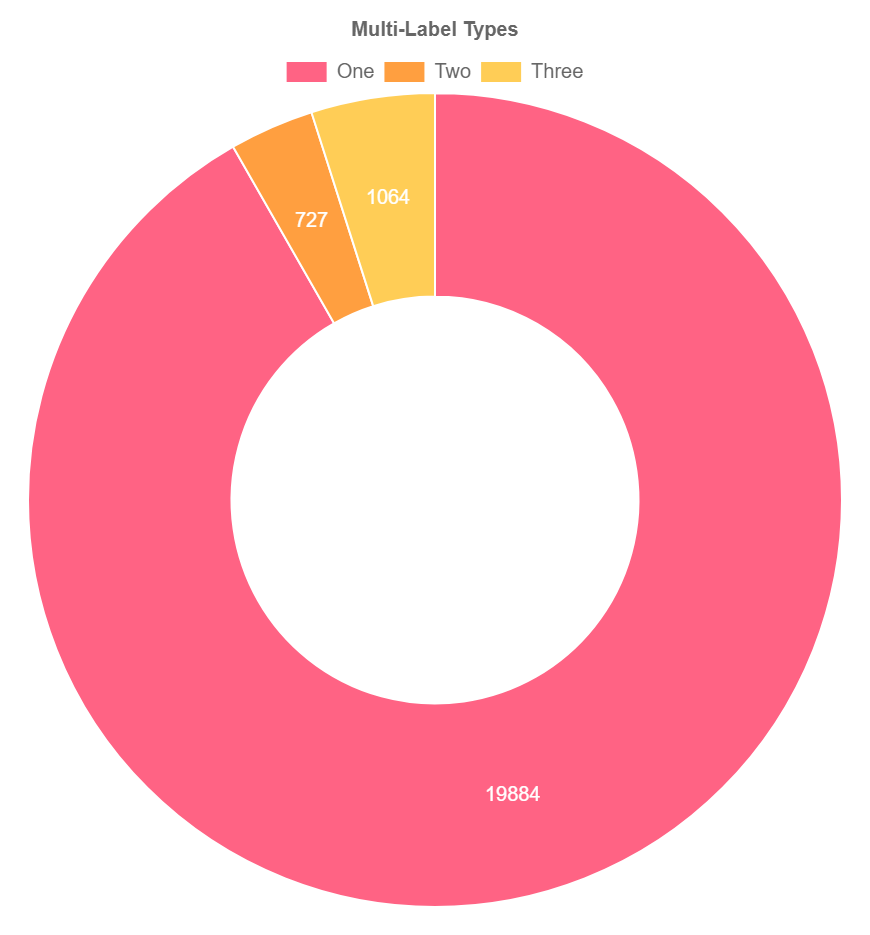
\includegraphics[width=\linewidth]{combined_db_label_types.png} 
	\caption{The proportion of each label type in the combined database.}
	\label{fig:combined_db_label_types}
\end{figure}

Each sample from a database would flow through the same preprocessing steps to maintain consistency. The preprocessing steps are
\begin{enumerate}
	\item The sample starts as a raw waveform in the form of time series points specifying the amplitude at a certain time.
	\item we then pad or crop the sample to a desired length. In our case, we set a maximum length of 4.5 seconds. Samples shorter than this were zero-padded on the right tail. Samples longer than this were cropped to this length and the extra information was discarded.
	\item If the sample came from a database that we considered noisy, then a noise reduction function was run on the sample to reduce the noise. We consider the IEMOCAP and CREMA-D databases to be noisy.
	\item The sample is then converted into a log-Mel spectrogram using a short-time Fourier transform (STFT) and Mel scale equation. The phase information was discard as it does not seem to hold relevant information. \cite{}
	\item The final step is to normalize the spectrograms to have values between negative one and one. This was done by using a minmax scaling function.
\end{enumerate}

\begin{figure}[h!]
	\centering
	\hspace{6mm}
	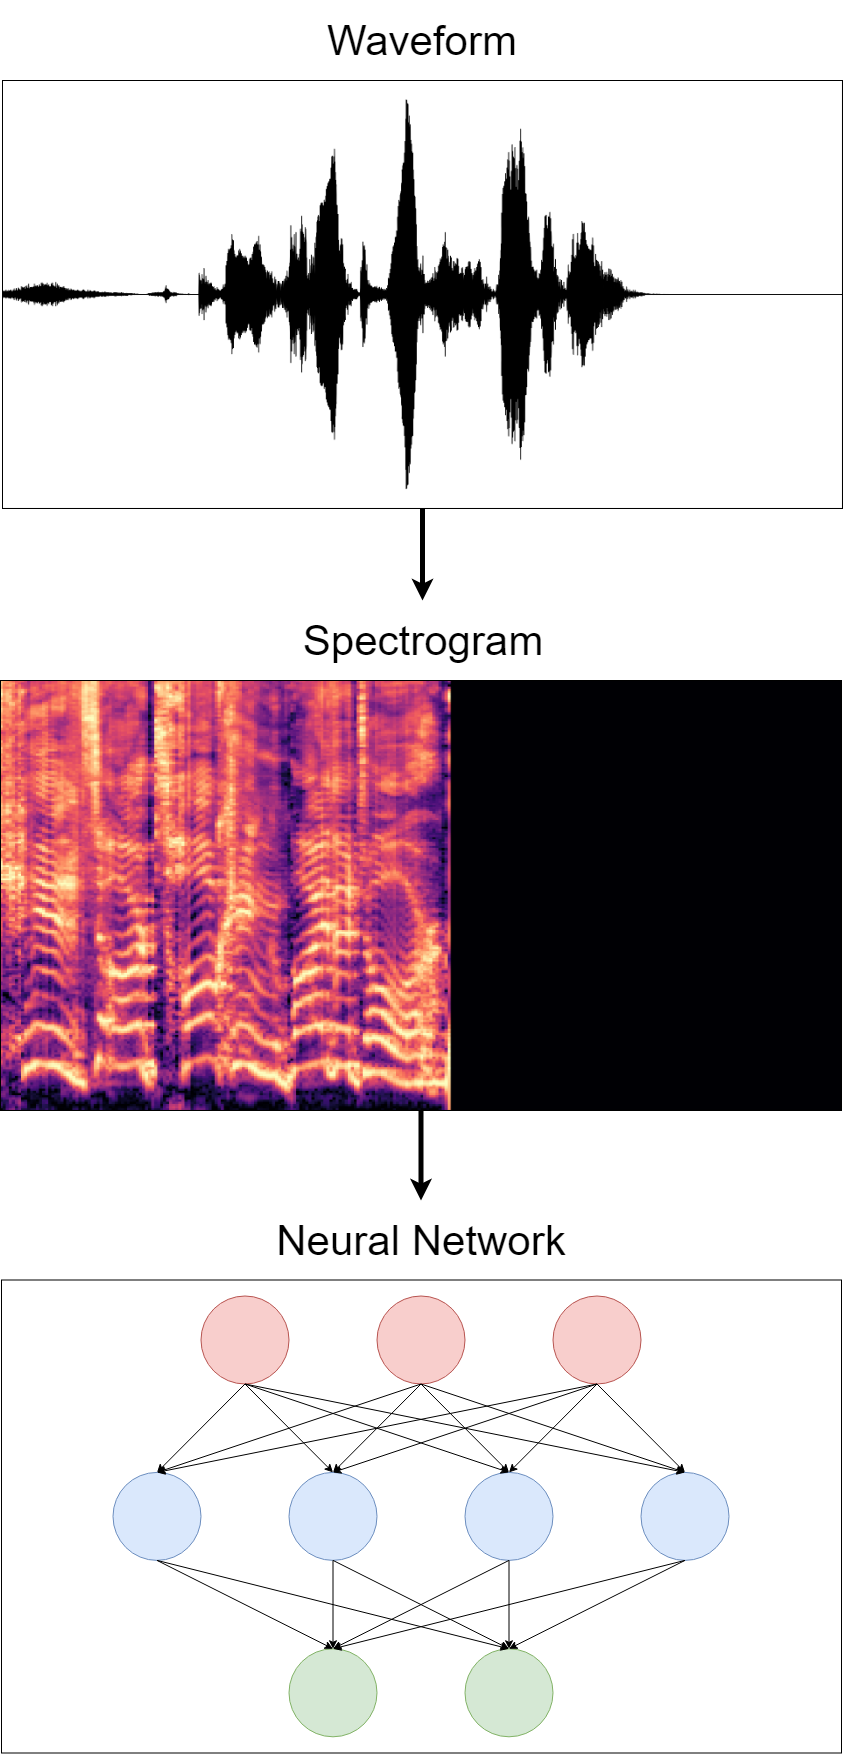
\includegraphics[width=\linewidth]{high_level_dataflow_diagram.png}
	\caption{A high level overview of the processing stages that a speech sample goes through.}
	\label{fig:high_level_dataflow_diagram}
\end{figure}

After all of the databases were processed this way, the final combined database was fed into a neural network for training. We constructed a seven layer neural network of four convolutional layers and three dense layers. The network architecture is shown in Figure \ref{label}. The training details follow.
\begin{itemize}
	\item We applied dropout to the dense layers and batch normalization to the convolutional layers to deal with overfitting.
	\item We shuffled the combined database to make each training batch more homogenous and thus prevent large gradient updates.
	\item We split the combined database into 80\% training, 10\% validation, and 10\% testing.
	\item We updated the model's hyperparameters based on the validation loss and accuracy to improve the model's accuracy and generalizability.
\end{itemize}

\begin{figure}[h!]
	\centering
	\hspace{6mm}
	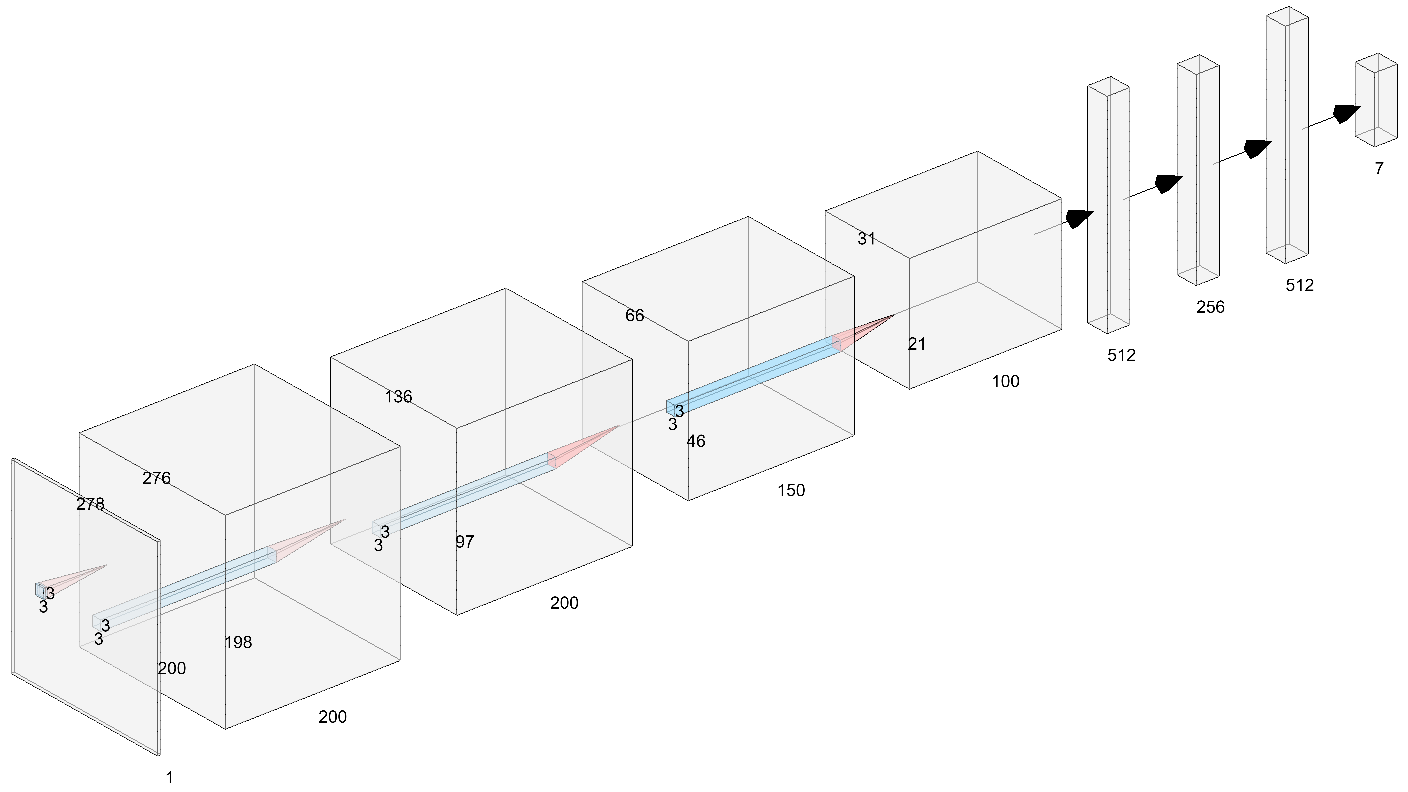
\includegraphics[width=\linewidth]{neural_network_architecture.png}
	\caption{The detailed architecture of the neural network including its eight layers and convolution filter size.}
	\label{fig:high_level_dataflow_diagram}
\end{figure}

\section{Results}

After training, the model was evaluated on the testing set to get the final accuracy of the model. The final accuracy achieved was 50\%. Confusion matrices for each emotion are shown in Figure \ref{}.

\section{Discussion}

\subsection{Results Summary}

We created a neural network model that achieved a classification accuracy of 50\% on the problem of multi-label emotion classification. This model can successfully classify multiple emotions in a sample and while this is a good result, we can do better.

\subsection{Limitations and Future Work}

One limitation of this work was that we only accounted for seven emotions but we know that there are more emotions than this. \cite{} Another limitations was that 
Here we present future improvements of our work 
\begin{itemize}
	\item Improving the recognition accuracy by using more sophisticated neural network architectures such as LSTMs or using more databases.
	\item Incorporating the phase data from the STFT and testing to see if that improves the accuracy.
	\item Testing a binary relevant approach to this multi-label problem and comparing it to this model.
\end{itemize}

\subsection{Conclusion}

Overall, this paper presented a convolutional neural network model that achieves a 50\% accuracy on multi-class, multi-label speech emotion recognition using four combined databases. We obtained this result by transforming raw speech samples into log-Mel spectrograms using STFT and the Mel scale. These log-Mel spectrograms are then fed into a eight layer neural network for classification for training. When we have completed training the neural network, the model was evaluated and achieved as 50\% accuracy. While this result is a promising start, we suggest improvements that future work can build upon to improve the accuracy.

\section*{Acknowledgment}
Acknowledge PURE award.


\bibliographystyle{IEEEtran}
\bibliography{IEEEabrv, references}

\end{document}
